\documentclass[12pt,a4paper]{article}
\usepackage[utf8]{inputenc} %polskie znaki
\usepackage[T1]{fontenc}	%polskie znaki
\usepackage{amsmath}		%matematyczne znaczki :3
\usepackage{enumerate}		%Dodatkowe opcje do funkcji enumerate
\usepackage{geometry} 		%Ustawianie marginesow
\usepackage{graphicx}		%Grafika
\usepackage{wrapfig}		%Grafika obok textu
\usepackage{float}			%Allows H in fugire
\usepackage{hyperref}		%Allows hyperlinks
%\pagestyle{empty} 			%usuwa nr strony
\usepackage{todonotes}		%Todo notatki
\usepackage{lipsum}         %Lorem text
\usepackage{ntheorem}   	% for theorem-like environments
\usepackage{mdframed}   	% for framing
\usepackage{subcaption}		% subfigure (image placing)
\usepackage{pdfcomment}		% Komentarze (z bazowego pdf'a)
\usepackage{xparse}			% New commands with optional arguments
\usepackage{ifthen}			% If then - funkcje!
\usepackage{expl3}			% Deklarowanie zmiennych
\usepackage{ulem}			% Przekreślone litery \sout{}

\newgeometry{tmargin=2cm, bmargin=2cm, lmargin=2cm, rmargin=2cm} 

%Counter commands{
	\newcounter{counter} % Creates a new counter
	\setcounter{counter}{1} % Sets the counter to 5
	\newcommand{\counter}[1]{
		\arabic{#1} \stepcounter{#1} 
	}
	\newcommand{\counterreset}[1]{\setcounter{#1}{1}}
	%}

%Define styles{
	\theoremstyle{break}
	\theoreminframepreskip{0.5cm}
	\theoremheaderfont{\bfseries}
	\newmdtheoremenv[%
	linecolor=white,%
	innertopmargin=\topskip,
	shadowsize=0,%
	innertopmargin=5,%
	innerbottommargin=5,%
	leftmargin=10,%
	rightmargin=10,%
	backgroundcolor=gray!20,%
	innertopmargin=0pt,%
	ntheorem]{zad}{Zadanie}
	
	\mdfdefinestyle{zadanie}{
		linecolor=white,%
		innertopmargin=5,%
		innerbottommargin=5,%
		leftmargin=10,%
		rightmargin=10,%
		backgroundcolor=gray!20,%
		innertopmargin=8,
		innerbottommargin=8,
		skipabove = 5,
	}
	\mdfdefinestyle{wzor}{
		linecolor=cyan,%
		linewidth=2pt,%
		innertopmargin=8,
		innerbottommargin=8,
		leftmargin=10,%
		rightmargin=10,%
		backgroundcolor = white, 
		fontcolor = black,
		skipabove = 5,
		skipbelow = 5,
	}
	%}

%Zadania templatex%{
	\newcommand{\Wzor}[1]{
		\begin{mdframed}[style=wzor]
			\centering #1
		\end{mdframed}
	}
	\newcommand{\ZadanieTextowe}[1]{
		\begin{mdframed}[style=zadanie]
			\textbf{Zadanie \counter{counter} } \\
			#1
		\end{mdframed}
	}
	\newcommand{\Zadanie}[2]{
		\ZadanieTextowe{#1}
		#2
	}
	\newcommand{\ZadanieABCD}[6]{
		\ZadanieTextowe{#1}
		#2 \\\\
		\begin{tabular}{p{7cm} p{7cm}}
			\textbf{A. }#3&
			\textbf{B. }#4\\\\
			\textbf{C. }#5&
			\textbf{D. }#6\\
		\end{tabular}
	}
	\newcommand{\ZadanieABCDEF}[8]{
		\ZadanieTextowe{#1}
		#2 \\\\
		\begin{tabular}{p{7cm} p{7cm}}
			\textbf{A. }#3&
			\textbf{B. }#4\\\\
			\textbf{C. }#5&
			\textbf{D. }#6\\\\
			\textbf{E. }#7&
			\textbf{F. }#8\\\\
		\end{tabular}
	}
	\newcommand{\Zadanietwoxtwo}[5]{
		\ZadanieTextowe{#1}
		\begin{tabular}{p{7cm} p{7cm}}
			\textbf{a)} #2&
			\textbf{b)} #3\\\\
			\textbf{c)} #4&
			\textbf{d)} #5\\\\
		\end{tabular}
	}
	\newcommand{\Zadanietwoxthree}[7]{
		\ZadanieTextowe{#1}
		\begin{tabular}{p{7cm} p{7cm}}
			\textbf{a)} #2&
			\textbf{b)} #3\\\\
			\textbf{c)} #4&
			\textbf{d)} #5\\\\
			\textbf{e)} #6&
			\textbf{f)} #7\\\\
		\end{tabular}
	}
	\newcommand{\Zadanietwoxfour}[9]{
		\ZadanieTextowe{#1}
		\begin{tabular}{p{7cm} p{7cm}}
			\textbf{a)} #2&
			\textbf{b)} #3\\\\
			\textbf{c)} #4&
			\textbf{d)} #5\\\\
			\textbf{e)} #6&
			\textbf{f)} #7\\\\
			\textbf{g)} #8&
			\textbf{h)} #9\\\\
		\end{tabular}
	}
	%}

\newcommand{\tg}{\text{tg}}
\newcommand{\ctg}{\text{ctg}}
\newcommand{\UkladRownan}[2]{
	$\left\{
	\begin{array}{l}
		#1 \\
		#2
	\end{array}
	\right.$
}

\begin{document}
	
	\begin{center}
		\LARGE Funkcja liniowa
	\end{center}

	\Zadanietwoxthree{Naszkicuj podane proste w \sout{kartezjańskim} układzie współrzędnych:}
	{$y=2x-3$}{$y=5$}
	{$y=\frac{2}{3}x+1$}{$y=-x-2$}
	{$y=-\frac{4}{5}x+3$}{$y=1\frac{1}{2}x-4$}
	
	\Zadanietwoxtwo{Przez które ćwiartki układu współrzędnych przechodzi podana prosta}
	{$y=3-2x$}{$y=\frac{1}{5}x+2$}
	{$y=\sqrt{3}x+\sqrt{2}$}{$y=(3\sqrt{2}-2\sqrt{3})x+(7-5\sqrt{2})$}
	
	\Zadanietwoxfour{Wyznacz prostą, przechodzącą przez punkty $A$ i $B$, gdzie}
	{$A=(-3,4)\qquad B=(1,0)$}{$A=(5,-1)\qquad B=(3,3)$}
	{$A=(5,6)\qquad B=(1,4)$}{$A=(2,3)\qquad B=(-1,-3)$}
	{$A=(4,-2)\qquad B=(-2,1)$}{$A=(4,-4)\qquad B=(-2,-4)$}
	{$A=(-1,-3)\qquad B=(3,2)$}{$A=(5,-1)\qquad B=(8,-10)$}
	
	\Zadanietwoxtwo{Określ monotoniczność prostej}
	{$y=\frac{2}{3}x-4$}{$y=-2x+5$}{$y=-7+8x$}{$\frac{1-\sqrt{2}}{3}x-4$}
	
	\Zadanietwoxtwo{Wyznacz parametr "m", dla którego prosta jest malejąca}
	{$y=(m-3)x+7+m$}{$y=5x+m+mx$}{$y=\frac{m+8}{5}x+\frac{3m-1}{7}$}{$y=(8-5m)x+\sqrt{3}m$}
	
	\Zadanietwoxtwo{Wyznacz miejsca zerowe funkcji}
	{$y=0,5x-2$}{$y=\frac{2-4x}{2}+2x-1$}
	{$y=7-2x$}{$y=\frac{1}{4}x+3\frac{1}{2}$}
	
	\Zadanietwoxtwo{Wyznacz parametr "k", dla którego podana prosta przechodzi przez punkt $P=(2,-3)$}
	{$y=2kx-3$}{$y=(2k+1)x+3k+2$}
	{$y=(2k-1)x+4x-5$}{$y=\frac{5k+2}{6}x-2k+1$}
	
	\newpage
	\begin{center}
		\LARGE Zadania maturalne
	\end{center}

	\counterreset{counter}
	\ZadanieABCD{Poniżej przedstawiono interpretację geometryczną układu równań.}
	{\begin{center}
			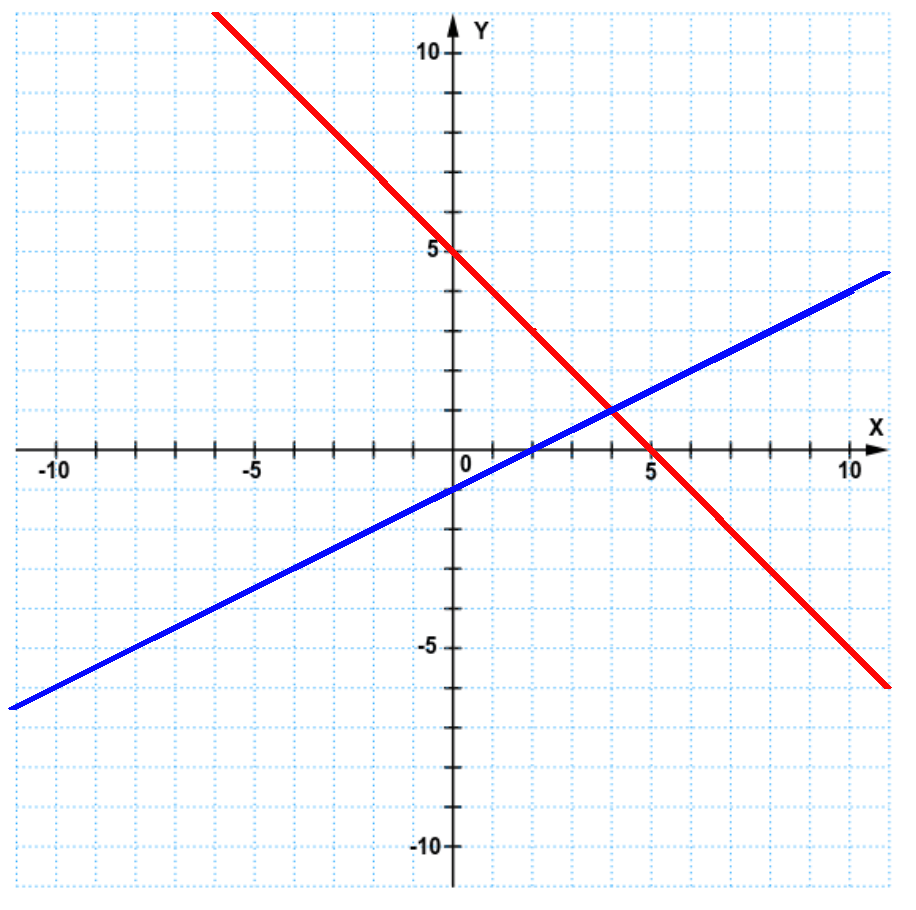
\includegraphics[scale=0.3]{3_1_1.png}
		\end{center}
		Układ ten da się zapisać w postaci}
	{\UkladRownan{y=x+5}{y=2x-1}}
	{\UkladRownan{y=-x+5}{y=2x+2}}
	{\UkladRownan{y=x-5}{y=\frac{1}{2}x-1}}
	{\UkladRownan{y=-x-5}{y=\frac{1}{2}x+2}}
	
	\ZadanieABCD{Dana jest funkcja liniowa określona wzorem
	$$y=(m^2-4)x+m-2$$}{nie ma miejsc zerowych kiedy}
	{m=2}{m=-2}
	{m=0}{m=$\sqrt{2}$}
	
	\Zadanie{Zapisz wartości parametru "m", dla którego funkcja
	$$y=(2m-3)x+3m-1$$
	jest niemalejąca.}{
	\vspace{0.5cm}	\dots\dots\dots\dots\dots\dots\dots\dots\dots\dots\dots\dots\dots\dots\dots\dots\dots\dots\dots\dots\dots\dots\dots\dots\dots\dots\dots\dots\dots\dots\dots}
	
\end{document}
